% my definition blocks

% Clement Elvira's colors
% \newenvironment{mydefblock}[1]{
%     \setbeamercolor{block title}{fg=white,bg=darkblue}
%     \setbeamercolor{block body}{fg=black,bg=bluegreen!10}
%     \begin{block}{#1}}{\end{block}}

% Toogle filled blocks
% \newenvironment{filledalertblock}[1]{
%     \metroset{block=fill}
%     \begin{alertblock}{#1}}{\end{alertblock}}

\newenvironment{mydefblock}[1]{%
    \metroset{block=fill}
    \begin{alertblock}{#1}}%
    {\end{alertblock}}

\newenvironment<>{mysotablock}[1][]{%
    % \setbeamercolor{block title}{fg=white,bg=darkblue}
    \setbeamercolor{postit}{fg=black,bg=bluegreen!10}
  \begin{beamercolorbox}[sep=.2em]{postit}#1}{\end{beamercolorbox}}

\newenvironment<>{mycontriblock}[1][]{%
  \setbeamercolor{postit}{fg=black,bg=mygreen!20}
  \begin{beamercolorbox}[sep=.2em]{postit}#1}{\end{beamercolorbox}}

\newenvironment<>{myfutureblock}[1][]{%
  \setbeamercolor{postit}{fg=myred,bg=mygreen!20}
  \begin{beamercolorbox}[sep=.2em]{postit}#1}{\end{beamercolorbox}}


\newcommand{\myThankTo}[1]{\textcolor{cyan}{(\faPeopleCarry~#1)}}

\newcommand{\rotate}[1]{\rotatebox[origin=c]{-120}{#1}}
\newcommand{\iconAOA}{\rotate{\faArrowsAltH}}
\newcommand{\iconDOA}{\faArrows*}
\newcommand{\iconAz}{\faArrowsAltH}
\newcommand{\iconEl}{\faArrowsAltV}
\newcommand{\iconAlert}{\faExclamationTriangle}
\renewcommand{\iconDNN}{%
    \leavevmode\unskip\penalty9999 \hbox{}\nobreak\hfill%
    \quad\hbox{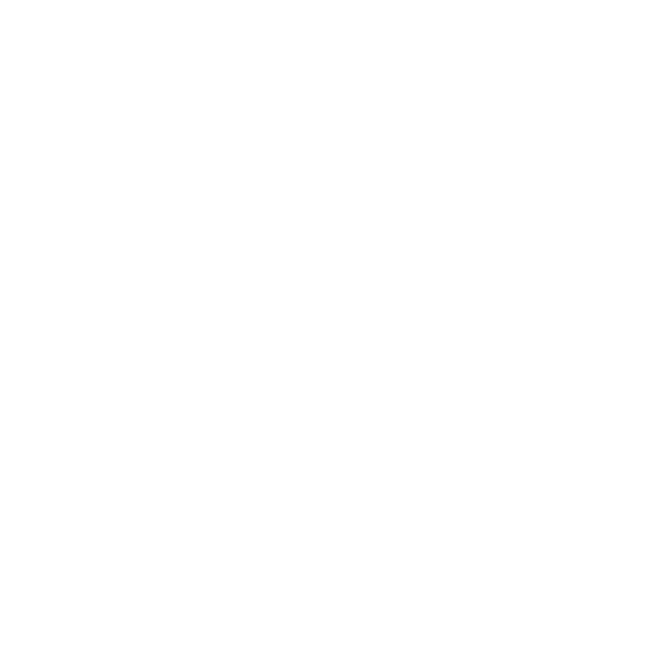
\includegraphics[height=1em]{figures/icon_dnn.png}}}

\newcommand{\pro}[1]{\textcolor{mygreen}{#1}}
\newcommand{\con}[1]{\textcolor{myred}{#1}}

\newcommand{\addendum}[1]{{\color{gray}\small (#1)}}

\newcommand{\mytriag}{\llap{\color{black!30}\scriptsize\raisebox{1pt}{$\blacktriangleright$}\quad}}

\newcommand{\blaster}{\alert{$\mathtt{Blaster}$}\xspace}
\newcommand{\lantern}{\alert{$\mathtt{Lantern}$}\xspace}
\newcommand{\dechorate}{\alert{$\mathtt{dEchorate}$}\xspace}
\newcommand{\brioche}{\alert{$\mathtt{Brioche}$}\xspace}
\newcommand{\mirage}{\alert{$\mathtt{Mirage}$}\xspace}
\newcommand{\separake}{\alert{$\mathtt{Separake}$}\xspace}

\newcommand{\cmark}{\textcolor{mygreen}{\ding{51}}}%
\newcommand{\xmark}{\textcolor{myred}{\ding{55}}}%

\newcommand{\aka}{\textit{a.k.a.}}
\newcommand{\eg}{\textit{e.g.}}
\newcommand{\ie}{\textit{i.e.}}

\newcommand{\RT}{\ensuremath{\mathtt{RT}_{60}}}
\newcommand{\SNR}{\ensuremath{\mathtt{SNR}}}

% MATH
\newcommand{\echoModelFreq}{\ensuremath{\sum_{r=0}^{R} \alpha_i^{(r)}(f) \cste^{- \csti 2 \pi \tau_i^{(r)} f_k}}}
\newcommand{\timeavg}{\ensuremath{\underset{t}{\mathtt{avg.}}}}


\usepackage{pgffor}
% for math stuff
\foreach \x in {a,...,z}{
  % mathbf
  \expandafter\xdef\csname bf\x \endcsname{\noexpand\ensuremath{\noexpand\mathbf{\x}}}
  % Bold symbol
  \expandafter\xdef\csname bs\x \endcsname{\noexpand\ensuremath{\noexpand\boldsymbol{\x}}}
  % Typewriter
  \expandafter\xdef\csname tt\x \endcsname{\noexpand\ensuremath{\noexpand\mathtt{\x}}}
  % mathfrak -- curly
  \expandafter\xdef\csname scr\x \endcsname{\noexpand\ensuremath{\noexpand\mathscr{\x}}}
  % short for \hat{}
  \expandafter\xdef\csname hat\x \endcsname{\noexpand\ensuremath{\noexpand\hat{\x}}}
  % short for \tilde{}
  \expandafter\xdef\csname tilde\x \endcsname{\noexpand\ensuremath{\noexpand\tilde{\x}}}
}

\foreach \x in {A,...,Z}{
%   Bold symbol -- bold
  \expandafter\xdef\csname bs\x \endcsname{\noexpand\ensuremath{\noexpand\boldsymbol{\x}}}
%   mathbf -- bold
  \expandafter\xdef\csname bf\x \endcsname{\noexpand\ensuremath{\noexpand\mathbf{\x}}}
%   mathbb -- blackboard-bold for uppercase letters and lowercase ( for sets )
  \expandafter\xdef\csname bb\x \endcsname{\noexpand\ensuremath{\noexpand\mathbb{\x}}}
%   mathds -- ???
  \expandafter\xdef\csname ds\x \endcsname{\noexpand\ensuremath{\noexpand\mathds{\x}}}
  % Typewriter
  \expandafter\xdef\csname tt\x \endcsname{\noexpand\ensuremath{\noexpand\mathtt{\x}}}
%   mathfrak -- gothic
  \expandafter\xdef\csname fk\x \endcsname{\noexpand\ensuremath{\noexpand\mathfrak{\x}}}
%   mathfrak -- curly
  \expandafter\xdef\csname scr\x \endcsname{\noexpand\ensuremath{\noexpand\mathscr{\x}}}
%   mathcal -- calligraphy
  \expandafter\xdef\csname cal\x \endcsname{\noexpand\ensuremath{\noexpand\mathcal{\x}}}
%   short for \hat{}
  \expandafter\xdef\csname hat\x \endcsname{\noexpand\ensuremath{\noexpand\hat{\x}}}
  % short for \tilde{}
  \expandafter\xdef\csname tilde\x \endcsname{\noexpand\ensuremath{\noexpand\tilde{\x}}}
}
